\label{chapter:correlatos}

Neste capítulo serão descritos os trabalhos que são relevantes, e de que forma eles contribuem ou diferenciam deste trabalho. Em específico, serão abordados as seguintes ferramentas: Valgrind Memcheck \cite{Nethercote:2007}, Symbtiotic 3 \cite{Chalupa:2016}, LEAKPOINT \cite{Clause:2010}, a versão anterior do Map2Check \cite{Rocha:2015} e o ESBMC \cite{Cordeiro:2012}. Todas essas feramentas verificam programas em C e são capazes de detectar violações em propriedades de segurança de memória, pode-se então criar um método analisando as vantagens e desvantagens de cada um desses trabalhos. 

\par
Valgrind é um \textit{framework} para instrumentação dinâmica em código binário (DBI). DBI são utilizados por ferramentas de \textit{Dynamic binary analysis} (DBA), onde o código de análise é instrumentado durante a execução, o que é conveniente pois o usuário não necessita recompilar o código. O módulo \textit{memcheck} é capaz de detectar violação de propriedades de segurança de memória utilizando \textit{shadow values}, \textit{bit} extra de rastreamento de endereços \cite{Nethercote:2007}, como descrito na \autoref{sub:dinamica}. Similarmente o Map2Check faz uso de instrumentação para verificar e validar propriedades de segurança de memória, porém o Map2Check não utiliza \textit{shadow values} para ocultar os registradores, a análise é feita anotando todas as operações de memória em uma estrutura. 

\par
\citeonline{Clause:2010} proporam uma maneira de detectar \textit{memory leaks} em programas em C e C$++$ (denominado de LEAKPOINT), de forma que obtenha informações para geração de contra-exemplos. O LEAKPOINT faz uma análise buscando funções de alocação (\texttt{malloc} e \texttt{new}) e liberação de memória (\texttt{free} e \texttt{delete}), além de operações com ponteiros, tudo isso em C e C$++$. Após isso, é feita uma análise se todas as instruções de alocação são desalocadas e se a aritmética de ponteiros está correta, caso seja verificado um problema, é possível informar com precisão onde ele ocorreu.

\par
O \textit{Extended SMT-Based Bounded Model Checker} (ESBMC) é um BMC baseado em satisfabilidade booleana (SAT) \cite{Cordeiro:2012}. O ESBMC é capaz de verificar programas em C com uma mais \textit{threads} e código com variáveis e \textit{locks} compartilhadas \cite{Morse:2013}. O ESBMC é capaz de ser utilizado para gerar propriedades de segurança de programas em C \cite{Rocha:2015}. 
%
O ESBMC Usa uma análise estática para aproximar para cada variável de ponteiro o conjunto de objetos de dados (isto é, blocos de memória) no qual este objeto poderia apontar para algum estágio na execução do programa. Os objetos de dados são numerados e um alvo de ponteiro é representado por um par de inteiros que identificam o objeto de dados e o deslocamento dentro do objeto. O valor de uma variável de ponteiro é então o conjunto de objetos (objeto, deslocamento) para o qual o ponteiro pode apontar na etapa de execução atual. O resultado de uma desreferência é a união dos conjuntos de valores associados a cada um dos objetos (objeto, \texttt{offset}). 


\par
O Symbiotic 3 \cite{Chalupa:2016} foi um protótipo criado utilizando execução simbólica com o Klee para encontrar violações de propriedades de segurança. O SYMBIOTIC 3 não utiliza um \textit{model checker} para gerar as propriedades de segurança, ele utiliza o Klee e um \textit{slicer}, pois a execução do Klee gera um espaço de estados muito grande.  Similarmente ao trabalho do \citeonline{Chalupa:2016}, a nova versão do Map2Check utlilizará o Klee para execução simbólica e um \textit{slicer}, e adicionalmente será utilizado um \textit{model checker} para gerar/inferir propriedades. A \autoref{fig:fluxoSymbiotic} exibe o fluxo do Symbiotic 3, pode-se observar que as saídas \textit{unknown} são feitas para caso a execução tenta verificar uma propriedade não suportada ou se uma instrução for uma que não seja suportada pelo Klee.

\begin{figure}[H]
	\caption{\label{fig:fluxoSymbiotic} Fluxo do Symbiotic 3}
	\begin{center}
	    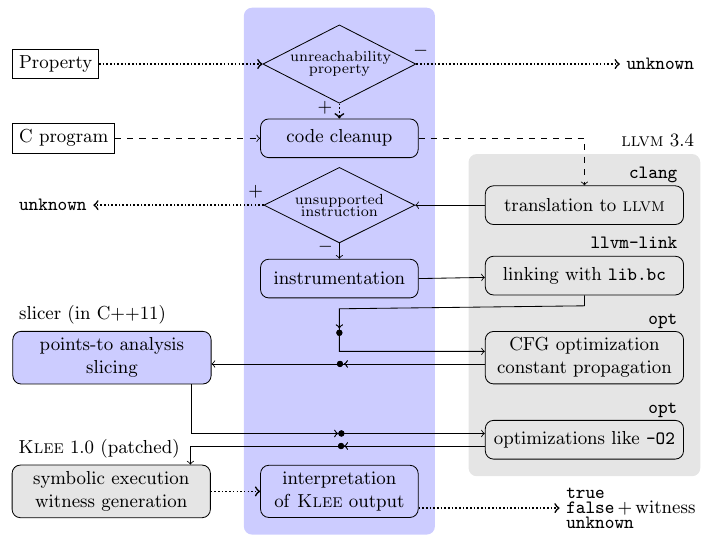
\includegraphics[scale=0.75]{resources/fluxoSymbiotic.png}
	\end{center}
	\legend{Fonte: \cite{Chalupa:2016}}
\end{figure}

\par
O \textit{Map2Check} \cite{Rocha:2015} é uma ferramenta criada para unir \textit{model checking} com \textit{teste unitário}, esta ferramenta gera assertivas utilizando ferramentas de \textit{bounded model checking} e depois as verifica utilizando CUnit por meio de uma biblioteca auxiliar para as assertivas. O foco do Map2Check é a linguagem C com o objetivo de observar e validar propriedades de segurança da memória. Este trabalho propõe estender o Map2Check substituindo a análise em cima do código C para um código em LLVM IR, e assim como Symbiotic 3 \cite{Chalupa:2016} fazendo uma execução simbólica utilizando o Klee juntamente com um \textit{slicer} para poder gerar as entradas para enfim validar as propriedades de segurança de ponteiros. Adicionalmente, assim como a versão anterior será integrado o ESBMC para geração de propriedades \cite{Rocha:2015}.

